\documentclass{article}

\usepackage{hyperref} % Zuerst hyperref laden
\usepackage{tocloft}
\usepackage[left=2.5cm,right=2.5cm,top=2.5cm,bottom=2.5cm]{geometry}
\usepackage{fancyhdr}
\usepackage{listings}
\usepackage{xcolor}
\usepackage{amsmath}
\usepackage{graphicx}
\usepackage{longtable}
\usepackage{tabu} % tabu als letztes laden



\pagestyle{fancy}
\fancyhf{}
\fancyhead[L]{Aufgabe 3}
\fancyhead[R]{Teilnehmer-ID:}
\fancyfoot[C]{\thepage}

\renewcommand{\cftsecleader}{\cftdotfill{\cftdotsep}}
\renewcommand*\contentsname{Inhaltsverzeichnis}

\title{\Huge{\textbf{Aufgabe 3 Siedler}} \\ \centering{\LARGE{Teilnahme-ID: ?????}}}
\author{Bearbeiter dieser Aufgabe: \\ Daniel Hohmann}
\date{\today}

\begin{document}

\thispagestyle{empty}
\begin{center}
\Huge{\textbf{Aufgabe 1 Siedler}}
\\
\LARGE{Teilnehmer-ID: ???}
\\
\LARGE{Bearbeiter dieser Aufgabe: \\ Daniel Hohmann}
\\
\LARGE{\today}
\end{center}
\newpage
\setcounter{page}{1}
\tableofcontents
\newpage
\section{\textcolor{blue}{Loesungsidee}}
\subsection{\textcolor{blue}{Geometrisches Optimierungsproblem}}
Bei der Aufgabe handelt es sich um ein Geometrisches optimierungsproblem. Wo das Problem darin liegt, den Besten Punkt innerhalb eines Polygons zu finden wo man ein Gesundheitszentrum erichten kann. Der Punkt muss die Bedingung erfuellen. Wenn ich ihn als mittelpunkt eines kreises benutze. Und ich ein radius von 85km um ihn herumziehe, und den kreis mit doerfern fuelle. Die alle einen abstand von 10km zueinander haben, und im Polygon liegen Damit sich die Krankheiten nicht uebertragen werden.
\\
Die naechste Aufgabe waere dann das Restliche Polygon noch mit doerfern zu fuellen fuer die aber gilt das sie einen abstand von 20km zueinander haben muessen.
\subsection{\textcolor{blue}{platzieren der Doerfer}}\label{sec:platzieren der Doerfer}
Wen ich den besten platz gefunden habe, kann ich die doerfer in abstaenden von 10km platzieren, indem ich bei einem radius von 10 anfange und bis zu einem radius von 80 hochzaehle in 10er schritten. Um nun die Punkte des Kreises zu berechen:
\vspace{5pt}
\hrule
\vspace{1.5pt}
\large{\textbf{Algorithmus umfang Punkte 1} Trigonomische funktionen}
\vspace{1.5pt}
\hrule
\begin{verbatim}
funktion punkte(centroid, polygon, distance)
	umfang_punkte = []
	for radius = 10 solange radius kleiner als 85 addiere zum radius 10
		umfang = 2 * pi * radius
		anzahl_punkte = (umfang/distance)
		
		for i solange i kleinr der anzahl_punkte addiere zu i 1
			winkel = (2 * pi * i)/anzahl_punkte
			x = centroid.x + radius * cos(winkel)
			y = centroid.y + radius * sin(winkel)
			wen der punkt(x,y) im polygon liegt
				umfang_punkte.append(punkt(x,y))
\end{verbatim}
\hrule
\vspace{5pt}
so bekommen wir die punkte die auf dem umkreis des kreises liegen. Um die Punkte fuer die naechsten Radin zu bestimmen, muessen wir legendlich den radius erhoehen um 10 solange bis wir bei 80 angekommen sind. So wie in dem pseudo code veranschaulicht. Um die restlichen Doerfer danach im abstand von 20km zu platzieren, kann ich auch die obrige funktion benutzen nur das ich eben bei dem radius von 100 anfange. Darduch ereiche ich das der abstand 20 ist und kann so weitermachen. Das einzige was ich im code noch ergaenzen muesste ist ein weiteres if-Statement das schaut ob der kreis noch das Polygon schneidet. Oder alternativ schauen ob ich noch ein punkt auf dem Polygon mit dem gegeben radius platzieren kann, wen nicht brich das Programm ab. Das wuerde mann dann aber eher mit einer while-do schleife realisieren. 
\subsubsection{\textcolor{blue}{Raycastalgorithmus}}
Ein wichtiges Problem was bis jezt entsteht ist, wie kann ich schauen ob eben ein Punkt innerhalb des Polygons liegt oder nicht?. das Problem kann man mit hilfe des raycastalgorithmus Behoben werden man schaut ob ein punkt innerhalb des Polygons liegt. Die funktions idee ist, das ich ein punkt habe und von diesem punkt aus versende ich strahlen(rays), dann schaue ich wie oft dieser strahl die kanten meines polygons schneidet. wenn die Anzahl ungrade ist, liegt der Punkt innerhalb des Polygons. Ist die annzahl jedoch Grade liegt der Punkt ausserhalb des Polygons. Das heisst gegeben muessen sein, mein Punkt den ich pruefen will $p(x_p|y_p)$ und mein Polygon \( \{ (x_i, y_i) \}_{i=0}^{n-1} \), hier steht $n$ fuer die anzahl der Eckpunkte.
\\
als naechstes inzinalisiere ich mein counter intersectionCount mit 0.
\\
Als naechstes lassen wir eine schleife ueber alle kanten des Polygons laufen, fuer jede kante des Polygons gilt $(P_i,P_i+1)$, wobei $P_i = (x_i,y_i)$, $P_i+1 = (x_i+1, y_i+1)$: 
\\
Jetzt ueberpruefen wir jede kante ob die horizontale linie durch $p$ schneidet.
\\
Danach Bestimmen wir die $y$-Koordinaten der Kantenenden: $y_i, y_i+1$.
\\
Nun ueberpruefen wir ob $p$ zwischen $P_i$ und $P_i+1$ liegt oder andersherum $(y_i > y_p) \neq (y_i+1 > y_p)$.
\\
Wenn nun die kannte die Horizontale linie schneidet berechne ich den $x$-wert des Schnittpunkts der kante $x_\text{intersect}$ was die horizontale Linie durch $p$ ist:
\\
$x_\text{intersect} = x_i + (y_i+1 - y_i)\frac{(x_i+1 - x_i) * (y_p - y_i)}{y_i+1 - y_i}$
\\
Als naechstes schauen wir das wenn $x_\text{intersect} > x_p$ zaehlen wir unseren intersectionCount um eins hoch.
\\
Zum schluss schauen wir dann wie hoch unser intersectionCount ist.  wenn er ungrade ist liegt der Punkt im Polygon ist der Grade liegt der Punkt nicht im polygon. Das sind alle wichtigen wesentlichen Funktionen, die fuer mein Algorithmus wichtig sind. zum visuellen verstaendnis habe ich noch eine veranschaulischungs Bild.
\\
\begin{figure}[h]
    \centering
    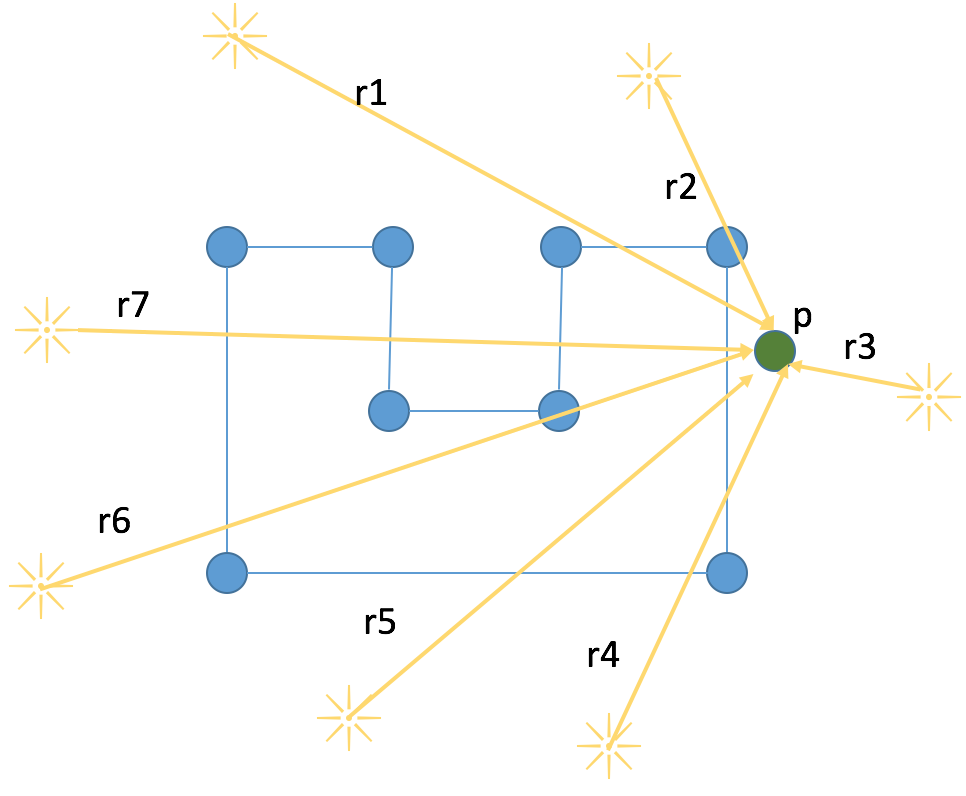
\includegraphics[width=0.7\textwidth]{Bilder/raycasting_polygon_3.png}
    \caption{Darstellung Raycastalgorithmus innerhalb eines Polygons, Quelle: https://kennycason.com/posts/2017-04-11-ray-casting.html}
    \label{fig:example}
\end{figure}

\subsection{\textcolor{blue}{Bruteforce}}
Der vermutlich einfachste weg der Mir einfaellt, waere es so lange zufaellige zahlen im bereich der min $x$,$y$ und max $x$,$y$ Koordinaten des Polygons zu generieren, bis man zweimal hintereinander Koordinaten generiert hat die wo sich der wert der punkte die innerhalb des Polygons liegen nicht aendert.
\vspace{5pt}
\hrule
\vspace{1.5pt}
\large{\textbf{Algorithmus 1} Brutforce}
\vspace{1.5pt}
\hrule
\begin{verbatim}
funktion brutforce(x,y)
	counter = 0
	do while true
		x = zufaelliger wert > min x && < max x
		y = zufaelliger wert > min y && max y
		counter = aufruf funktion zum Berechnen der anzahl der Punkte(x,y)
		
		wenn counter == counter, zweimal hintereinander
		return x,y 
\end{verbatim}
\hrule
\vspace{5pt}
Das Problem an dem ansatz ist natuerlich das ich wen ich pech habe zweimal den gleichen Punkt bekomme, oder aber ein punkt der sehr nahe am anderen liegt. Und der algorithmus deshalb nicht funktioniert. Abgesehen davon haben wir im worst case eine extrem lange laufzeit.
\subsection{\textcolor{blue}{Innenkreis}}
eine Theoretisch bessere Idee die ich gefunden habe, ist es den innenkreis eines Polygons zu Berechnen. Der Innenkreis eines Polygons ist der kreis, mit dem groest moeglichen radius der innerhalb eines polygons liegt. Das Problem daran ist aber, das es nur bei regelmaessigen Polygonen funktioniert. Und bei unregelmaessigen Polygonen sogut wie unmoeglich ist den Innenkreis zu berechnen. damit ist die Idee sofort weckgefallen da min. zwei der Bsp. Polygone unregelmaessig sind.
\subsection{\textcolor{blue}{Raster algorithmus}}
Ein weitaus besserer ansatz war meiner meinung nach der Rasteralgorithmus. Also ein Raster ueber das Polygon zu legen, und dann einfach den Punkt zu finden der am meisten Punkte mit einem radius von 85 Einheiten halten kann.
\vspace{5pt}
\hrule
\vspace{1.5pt}
\large{\textbf{Algorithmus 2} Raster}
\vspace{1.5pt}
\hrule
\begin{verbatim}
funktion raster(polygon)
	points_x = []
	points_y = []
	x_werte = []
	y_werte = []
	for i in reichweite anzahl x werte der kanten des polygon
		x_werte.append(polygon.x)
	for i in reichweite anzahl y werte der kanten des polygon
		y_werte.append(polygon.y)
	min_x = min(x_werte)
	min_y = min(y_werte)
	max_x = max(x_werte)
	max_y = max(y_werte)
	
	for min_x in reichweite max_x step Bsp. 10
		points_x.append(min_x)
	for min_y in reichweite max_y step Bsp. 10
		points_x.append(min_y)
		
	jezt nur noch schauen ob der punkt im polygon liegt wen ja lass ihn in der liste wenn
	nein nimm ihn raus 
\end{verbatim}
\hrule
\vspace{5pt}
Am ende erhalten wir ein raster von Punkten, die ueber das Polygon im abstand von 10 Einheiten verteilt sind. jetzt koennte man die punkte alle durchgehen, und schauen welcher punkt die meisten punkte im radius von 85 Einheiten halten kann, und diesen punkt als Gesundheitszentrum setzen. Das Problem an diesem Ansatz ist das je geanuer wir den optimalen punkt haben wollen, desto kleiner muss der abstand zwischen den Rasterpunkten werden. Je kleiner die Rasterpunkte werden je laenger dauert es sie alle durch zu iterieren. Das heist im volgeschluss das der Algorithmus nur fuer kleinste Polygone geeignet waere wenn ueberhaupt.

\subsection{\textcolor{blue}{End Algorithmus idee}}
Meine End idee um den bestenpunkt innerhalb des Polygons zu suchen um das Gesundheitszentrum zu platzieren ist, Ich fange an den centroid zu bestimmen. Warum der centroid weil der centroid der masseschwerpunkt eines objektes ist. Im fall des polygons ist es zwar nur eine annaeherung aber wir bekommen trozdem jedes mal einen relativ centralen punkt Innerhalb des Polygons. um den centroid zu berechnen benutzen wir einfach die Formel:
\[
\text{area} = \frac{1}{2} \left| \sum_{i=1}^{n} (x_i y_{i+1} - x_{i+1} y_i) \right|
\]
\\
Hierbei wird $P_{n+1}$ als $P_1$ behandelt, d.h., $x_{n+1} = x_1$ und $y_{n+1} = y_1$.
\\
Der Schwerpunkt $(cx, cy)$ des Polygons wird dann berechnet als:

\[
cx = \frac{1}{6 \cdot \text{area}} \sum_{i=0}^{n-1} (x_i + x_{i+1}) \cdot (x_i y_{i+1} - x_{i+1} y_i)
\]
\[
cy = \frac{1}{6 \cdot \text{area}} \sum_{i=0}^{n-1} (y_i + y_{i+1}) \cdot (x_i y_{i+1} - x_{i+1} y_i)
\]

Hierbei wird $P_{n}$ als $P_0$ behandelt, d.h., $x_{n} = x_0$ und $y_{n} = y_0$.
\\
Damit erhalten wir die $x$,$y$-Koordinaten, des centroid den wir als unser startwert fuer unseres Gesundheitszentrum verwenden. Danach berechnen wir alle Punkte fuer jeden radius wie in kapitel \ref{sec:platzieren der Doerfer} platzieren der Doerfer erklaert. Danach Iteriere ich durch alle punkte durch die wir bekommen habe, und ich rufe fuer jeden punkt wieder die funktion auf. Und schaue ob der punkt mehr punkte halten kann als der startpunkt. Wenn ja wird das mein neuer startpunkt sobald ich damit durch bin mache ich das gleiche nochmal aber diesesmal fuer den neuen starpunkt das Ganze wiederhole ich solange bis ich zweimal hintereinander den gleichen wert erhalte. das heist dann ja das ich nicht mehr den punkt optimieren kann. mit dieser methode sollte ich mich sehr nahe an den perfekten punkt fuer unser Gesundheitszentrum annaehern.
\\
Um die restlichen punkte zu platzieren mache ich wieder das prinzip wie im kapitel \ref{sec:platzieren der Doerfer} platzieren der Doerfer. und breche die schleife zum platzieren dann ab wenn ich kein punkt mehr im polygon platzieren kann.
\\
Als erweiterung ist mir direkt eingefallen das man das ganze plotten kann und auch eigendlich sollte da man sonst beim Programmieren, beim endregebnis probleme hat das ganze nachzuvollziehen und wirklich zu ueberpruefen und zu verstehen. Da ich Das ganze in C++ werde ich die libary Matplotlibcpp benutzen da es die in meinen gen beste option dafauer ist.
\\
Das Problem was ich an dieser Methode sehe ist wie oben schon angedeutet, das es nur eine annaerung ist und nicht der perfekte oder optimalste punkt ueberhaupt. zudem kann es je nach groesse des polygons zu laengeren berechnungen kommen. auch ein grund warum ich fuer das Projekt am ende C++ benutzt habe.

\subsection{\textcolor{blue}{Quellen:}}
\begin{itemize}
\item[\normalsize{[1]}] \normalsize{Raycasting, https://de.wikipedia.org/wiki/Raycasting}
\item[\normalsize{[2]}] \normalsize{Checking if a point is inside a polygon is RIDICULOUSLY simple (Ray casting algorithm) - Inside code (YouTube video), https://www.youtube.com/watch?v=RSXM9bgqxJM}
\item[\normalsize{[3]}] \normalsize{Inkreis regelmäßiges Polygon, https://www.maths2mind.com/schluesselwoerter/inkreis-regelmaessiges-polygon}
\item[\normalsize{[4]}] \normalsize{Inkreis, https://de.wikipedia.org/wiki/Inkreis}
\end{itemize}
\section{\textcolor{blue}{Umsetzung}}
\subsection{\textcolor{blue}{Algeimeine Hinweise zur Benutzung}}
Das programm ist wie eben Schon angedeutet in der Programmiersprache C++ 13.2.0 implementriert, und unter Debian(linux) getestet. zum visuallisieren der Polygone und der Doerfer(punkten), Kommt hier die Libary Matplotlib zum einsatz eine uhrspruenglich fuer Python entwickelte libary. Um sie in c++ zu benutzen, benutze ich die header file matplotlibcpp.h$^1$ von Julien Gacon die durch embedded python zugriff auf diese libary bietet.
\\
zum Benutzen der libary ist eine instalation von Python und der libary matplotlib(sudo pip3 install matplotlib) vorauszusetzen.
\\
Die Eingabe erfolgt ueber die programm datei selbst indem man den path zu der gewuenschten datei setzt.Die Ausgabe wiederum erfolgt ueber das Terminal.
\\
 Das ware auch Gleich schon eine optimierungs idee fuer die Zukunft, das man die Ausgabe in eine datei macht und den input ueber das Termianl.
\vspace{5pt}
\hrule
\begin{itemize}
\item[$^1$] \text{https://github.com/Cryoris/matplotlib-cpp/blob/master/matplotlibcpp.h}
\end{itemize}
\subsection{\textcolor{blue}{Die datei \text{\normalsize{Geometrie.h}}}}
Die Datei \texttt{Geometrie.h} enthaelt zwei klassen die Klasse Point und die Klasse Polygon. Die funktionen dieser Objekte treten recht haufig innerhalb des Quellcodes auf da sie essenzielle algorithmen wie den raycastalgorithmus enthalten. Hier eine Uebersicht ueber die Funktionen.
\par\medskip
\begin{center}\Large{ Polygon}\end{center}
\begin{longtable}{|>{\raggedright\arraybackslash}p{3.5cm}|p{11.5cm}|}
\hline
\textbf{Funktion} & \textbf{Beschreibung} \\
\hline
\endfirsthead
\hline
\textbf{Funktion} & \textbf{Beschreibung} \\
\hline
\endhead
\texttt{isInsidePolygon()} &
Ueberprueft ob ein Punkt innerhalb des Gegebenen Polygons liegt. mithilfe eines raycastalgorihmuses. Der von einem Punkt einen strahl schiesst, und schaut wie oft er die Kanten des Polygons schneidet. Wenn die Anzahl ungrade ist liegt der Punkt innerhalb des Polygons ist die Zahl grade liegt er ausserhalb. \\
\hline
% Weitere Zeilen hier einfügen...
\end{longtable}

\section{\textcolor{blue}{Beispiele}}
\section{\textcolor{blue}{Quellcode}}
\end{document}